\section{Experimental Set-Up} \label{sec:experiment}

This section presents all experimentation details. Starting with what was done for data preparation, then identifying the network architecture and parameters, then explaining experiment runs and how results were captured.

\subsection{Data Preparation}
As mentioned in Section \ref{sec:domain}, the dataset consists of 512x512 images of one or more fruits. In addition, the data set provides labels for the images in the form of a class and the top-left coordinates, height and width of the associated bounding box. In pre-processing the data, we created a data frame wherein the height and width attributes were replaced with the bottom-right coordinates of the bounding box. In addition, we replaced the class labels as follows:
\begin{itemize}
    \item \emph{fruit\_brownspot} would be replaced with 1.
    \item \emph{fruit\_brownspot} would be replaced with 2.
    \item \emph{fruit\_brownspot} would be replaced with 3.
\end{itemize}

Consequently, the following represents a sample of what the data labels looked like at this stage:

\begin{figure}[htbp]
\centerline{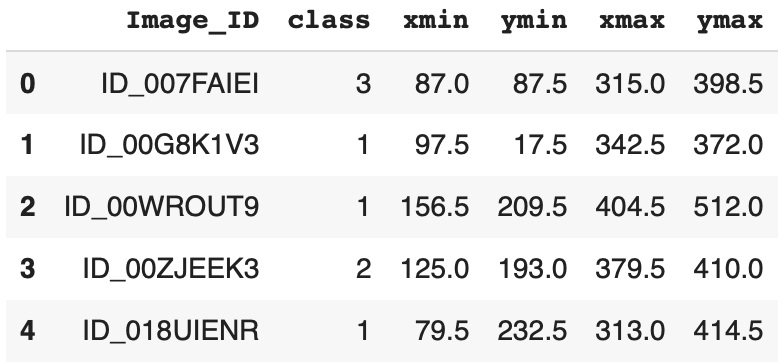
\includegraphics[width=0.5\textwidth]{report/4_experimental/data.png}}
\caption{Image labels after pre-processing.}
\label{fig:data}
\end{figure}

Next, we performed binary one-hot encoding on the classes and scaled the image data itself such that all data was scaled between 0 and 1. This was done because it is required by the Keras \cite{keras} implementation of ResNet50V2 \cite{ResNet50V2}, which we would be using.

Finally, we performed an 80/20 split between the training data and validation data. No split was performed for test data because the competition provided an entirely separate data set for testing purposes.

\subsection{Network Parameters}

For the purposes of this report, we made use of a convolutional neural network architecture which uses ResNet50V2 \cite{ResNet50V2} for the feature extraction segment of the network. In other words, the network comprised a combination of ResNet50V2 \cite{ResNet50V2} - which would not be trained - and 2 branches - one for classifying classes for fruits, and another for identifying bounding boxes.

Each of the 2 branches had one input layer, and single hidden layer and a single output layer. The branch for classifying fruit classes also included 2 dropout layers. For activation functions for the different layers, we made use of ReLU, Sigmoid and Softmax functions. 

For the size of the the first and second layers of each branch - and, for the learning rate - we performed hyperparameter tuning using teh Hyperband Tuner \cite{hyperband}. Following tuning, this was the best hyper-parameter compination that could be found:
\begin{itemize}
    \item \emph{Number of units in the first layer of each branch}: 48
    \item \emph{Number of units in the second layer of each branch}: 32
    \item \emph{Learning rate:} 0.0001
\end{itemize}

\subsection{Running Experiments} \label{sec:experiment_run}
Firstly, note that all experiments were executed using  the Tensorflow framework and the Keras high-level API \cite{keras}. For each of the optimisation and training methods considered, we performed 10 runs. Each run consists of training the network from scratch, for 10 epochs, and testing the networks performance against the test data set.

After 10 test runs had been completed, we calculated the average and standard deviation of the training and validation accuracies across all runs. Additionally, we calculated the average accuracy and sparse categorical crossentropy loss for the test data set across the 10 runs.

All code used to run experiments is available at https://github.com/marcus-bornman/cos\_711\_assignment\_3.